% Preamble
\documentclass[10pt,letterpaper]{article}
\usepackage[spanish]{babel}

% Packages
\selectlanguage{spanish}
\usepackage[utf8]{inputenc} % For spanish (and international) letters like acents.
\usepackage{hyperref} % To create hyperlinks within the document.
\hypersetup{ % Custome options for package hyperref:
	colorlinks=true, % Links without borders
	linkcolor=black, % Internal links (black index)
	urlcolor=blue % External links
}
\usepackage{graphicx} % To include graphics (pictures, images)
\usepackage{float} % For the use of the parameter "H" in command "\begin{figure}[H]" (i.e. exact position of image in text)
\usepackage{tabularx} % Similar to tabular* environment, for width and stretching in tables
\usepackage[table]{xcolor} % Color in cell [http://ctan.org/pkg/xcolor]
\definecolor{NewBlue}{RGB}{102, 153, 255}
\usepackage[strict]{changepage} % Allow to change margins (like \textwidth). 
% By the way, about page size and margins: https://www.sharelatex.com/learn/Page_size_and_margins

% Document environment
\begin{document}

% Top matter
\title{Documentación de los Requerimientos del Sistema de apoyo a la catalogación de archivos audiovisuales del LAIS}
\author{Rodrigo Eduardo Colín Rivera, Sergio Amaro Rosas}
\date{\today}
\maketitle

\begin{abstract}
La siguiente documentación tiene como objetivo \ldots
\end{abstract}

\tableofcontents % Indice
\newpage

\setcounter{secnumdepth}{0} % Non-numbering sections
\setcounter{tocdepth}{0} % Non-numnbering table of contents
\graphicspath{{../Diagramas/}{../Screenshots}} % Path of the folders containing the images

\section{Enunciado del problema}

\section{Diagrama general de casos de uso}
\begin{figure}[H]
	\centering
	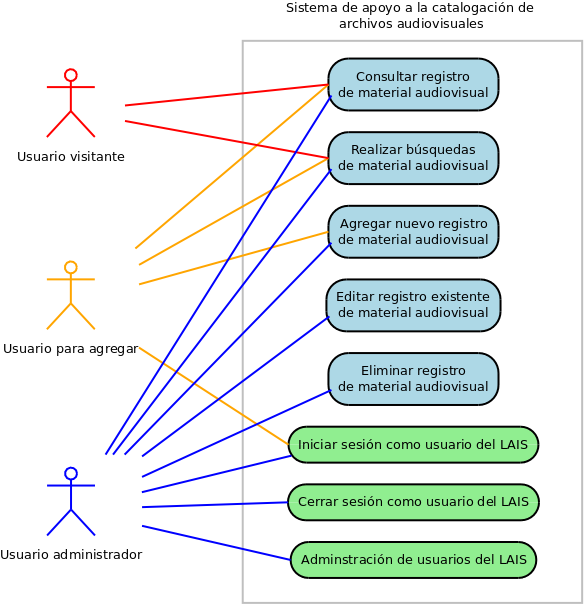
\includegraphics[width=0.8\textwidth]{CasosDeUso.png}
	\caption{Diagrama de casos de uso}
	\label{fig:caso_de_uso}
\end{figure}

\section{Casos de uso detallados, casos de prueba, prototipo de interfaz}

\subsection{Usuario visitante}

\subsubsection{Consultar información de archivo audiovisual}
% Actor
\textbf{Actor:} Usuario visitante

% Imagen del diagrama específico del caso
\begin{figure}[H]
	\centering
	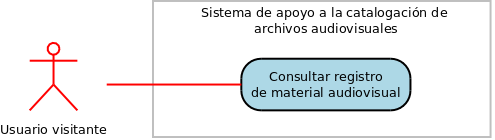
\includegraphics[width=0.8\textwidth]{CasoDeUso_Visitante_ConsultarRegistro.png}
\end{figure}

% Descripción
\textbf{Descipción: } Acción que permite mostrar la información completa de un archivo audiovisual cuya portada es mostrada en pantalla.

% Precondiciones
\textbf{Precondiciones:} Estar en alguna de las páginas que muestra los archivos audiovisuales por década.

% Flujo Normal de Eventos (tabla)
\begin{adjustwidth}{-6em}{-6em}
	\begin{center}
		\begin{tabularx}{1.2\textwidth}{ | p{0.7cm} | X | p{0.7cm} | X | p{1.5cm} | }
			\hline
			\rowcolor{NewBlue} \multicolumn{5}{|c|}{\textbf{Flujo normal de eventos}} \\
			\hline
			\multicolumn{2}{|c|}{\textbf{Actor(es)}}	&	\multicolumn{2}{c|}{\textbf{Sistema}}	&	\textbf{Alterno} \\
			\hline
			\textbf{Paso}	&	\textbf{Acción}	&	\textbf{Paso}	&	\textbf{Acción}	&	\textbf{ID} \\
			\hline
			1 & 
			Dar clic en la portada del audiovisual que se desea ver &
			2 &
			El sistema pide todos los datos del audiovisual a la base de datos &
			E1 \\
			\hline
			& 
			&
			3 &
			El sistema muestra una ventana emergente con toda la información del audiovisual. & 
			A1 \\
			\hline
		\end{tabularx}
	\end{center}
\end{adjustwidth}

% Flujo Alterno (en caso de ser necesario)
\begin{adjustwidth}{-6em}{-6em}
	\begin{center}
		\begin{tabularx}{1.2\textwidth}{ | p{0.6cm} | X | X | }
			\hline
			\rowcolor{NewBlue} \multicolumn{3}{|c|}{\textbf{Flujo alterno de eventos}} \\
			\hline
			\textbf{ID}	&	\textbf{Descripción}	&	\textbf{Acción} \\
			\hline
			A1 &
			El usuario da clic en el botón de ``Ver más'' para ver información específica del archivo audiovisual &
			El sistema muestra en la parte inferior toda la información disponible del archivo audiovisual separada por áreas. \\
			\hline
		\end{tabularx}
	\end{center}
\end{adjustwidth}

% Flujo de Excepcion de Eventos (tabla)
\begin{adjustwidth}{-6em}{-6em}
	\begin{center}
		\begin{tabularx}{1.2\textwidth}{ | p{0.6cm} | X | X | }
			\hline
			\rowcolor{NewBlue} \multicolumn{3}{|c|}{\textbf{Flujo excepcional de eventos}} \\
			\hline
			\textbf{ID}	&	\textbf{Descripción}	&	\textbf{Acción} \\
			\hline
			E1 &
			No hay conexión con la base de datos. &
			El sistema devuelve un mensaje de error de conexión. \\
			\hline
		\end{tabularx}
	\end{center}
\end{adjustwidth}

% Post-condiciones
\textbf{Postcondiciones:} El entorno de la página se oscurece para dar enfoque a la información completa del archivo audiovisual.

% Casos de prueba para flujo normal (tabla) y su prototipo (imagen)
%\begin{figure}[H]
%	\centering
%	\includegraphics[width=0.8\textwidth]{imagen.png}
%\end{figure}

\begin{adjustwidth}{-6em}{-6em}
	\begin{center}
		\begin{tabularx}{1.2\textwidth}{ | X | X | }
			\hline
			\rowcolor{NewBlue} \multicolumn{2}{|c|}{\textbf{Casos de prueba (Flujo normal)}} \\
			\hline
			\textbf{Entradas}	&	\textbf{Resultado esperado} \\
			\hline
			Clic en una portada de audiovisual. &
			Mostrar el contenido completo del archivo audiovisual seleccionado. \\
			\hline
		\end{tabularx}
	\end{center}
\end{adjustwidth}

% Casos de prueba (Flujo alterno de eventos) [cuando es necesario]

%\begin{figure}[H]
%	\centering
%	\includegraphics[width=0.8\textwidth]{imagen.png}
%\end{figure}

\begin{adjustwidth}{-6em}{-6em}
	\begin{center}
		\begin{tabularx}{1.2\textwidth}{ | p{0.6cm} | X | X | }
			\hline
			\rowcolor{NewBlue} \multicolumn{3}{|c|}{\textbf{Caso de prueba (Flujo alterno)}} \\
			\hline
			\textbf{ID}	&	\textbf{Entrada}	&	\textbf{Resultado esperado} \\
			\hline
			A1 &
			Clic en el botón de ``Ver más''. &
			El sistema muestra en la parte inferior toda la información disponible del archivo audiovisual separada por áreas. \\
			\hline
		\end{tabularx}
	\end{center}
\end{adjustwidth}

% Casos de prueba para excepción de eventos (tabla) y su prototipo (imagen)
%\begin{figure}[H]
%	\centering
%	\includegraphics[width=0.8\textwidth]{imagen.png}
%\end{figure}

\begin{adjustwidth}{-6em}{-6em}
	\begin{center}
		\begin{tabularx}{1.2\textwidth}{ | p{0.6cm} | X | X | }
			\hline
			\rowcolor{NewBlue} \multicolumn{3}{|c|}{\textbf{Caso de prueba (Flujo excepcional)}} \\
			\hline
			\textbf{ID}	&	\textbf{Entrada}	&	\textbf{Resultado esperado} \\
			\hline
			E1 &
			Clic en una portada de audiovisual. &
			El sistema devuelve un mensaje de error de conexión. \\
			\hline
		\end{tabularx}
	\end{center}
\end{adjustwidth}

\subsubsection{Realizar búsqueda de material audiovisual}
% Actor
\textbf{Actor:} Usuario visitante

% Imagen del diagrama específico del caso
\begin{figure}[H]
	\centering
	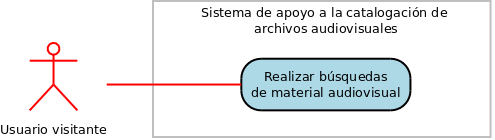
\includegraphics[width=0.8\textwidth]{CasoDeUso_Visitante_Busqueda.png}
\end{figure}

% Descripción
\textbf{Descipción: } Acción que permite realizar una búsqueda de material audiovisual.

% Precondiciones
\textbf{Precondiciones:} Estar en cualquiera de las páginas del sistema.

% Flujo Normal de Eventos (tabla)
\begin{adjustwidth}{-6em}{-6em}
	\begin{center}
		\begin{tabularx}{1.2\textwidth}{ | p{0.7cm} | X | p{0.7cm} | X | p{1.5cm} | }
			\hline
			\rowcolor{NewBlue} \multicolumn{5}{|c|}{\textbf{Flujo normal de eventos}} \\
			\hline
			\multicolumn{2}{|c|}{\textbf{Actor(es)}}	&	\multicolumn{2}{c|}{\textbf{Sistema}}	&	\textbf{Alterno} \\
			\hline
			\textbf{Paso}	&	\textbf{Acción}	&	\textbf{Paso}	&	\textbf{Acción}	&	\textbf{ID} \\
			\hline
			1 & 
			Escribir texto de búsqueda en el campo situado en la parte superior del navegador y presionar \textit{Enter} en el teclado o clic en el botón con el icono de lupa situado a la derecha &
			2 &
			El sistema realiza una búsqueda dentro de la base de datos con las coincidencias de las palabras escritas &
			E1 \\
			\hline
			& 
			&
			3 &
			El sistema muestra los resultados en pantalla utilizando la misma vista que los archivos audiovisuales por década (mostrando la portada, el título y el año) & 
			E2\\
			\hline
		\end{tabularx}
	\end{center}
\end{adjustwidth}

% Flujo de Excepcion de Eventos (tabla)
\begin{adjustwidth}{-6em}{-6em}
	\begin{center}
		\begin{tabularx}{1.2\textwidth}{ | p{0.6cm} | X | X | }
			\hline
			\rowcolor{NewBlue} \multicolumn{3}{|c|}{\textbf{Flujo excepcional de eventos}} \\
			\hline
			\textbf{ID}	&	\textbf{Descripción}	&	\textbf{Acción} \\
			\hline
			E1 &
			No hay conexión con la base de datos. &
			El sistema devuelve un mensaje de error de conexión. \\
			\hline
			E2 &
			No hay coincidencias de búsqueda en la base de datos. &
			El sistema muestra un texto indicando no hay resultados de la búsqueda. \\
			\hline
		\end{tabularx}
	\end{center}
\end{adjustwidth}

% Post-condiciones
\textbf{Postcondiciones:} El usuario es autodirigido a la página que muestra los audiovisuales resultantes de la búsqueda.

% Casos de prueba para flujo normal (tabla) y su prototipo (imagen)
%\begin{figure}[H]
%	\centering
%	\includegraphics[width=0.8\textwidth]{imagen.png}
%\end{figure}

\begin{adjustwidth}{-6em}{-6em}
	\begin{center}
		\begin{tabularx}{1.2\textwidth}{ | X | X | }
			\hline
			\rowcolor{NewBlue} \multicolumn{2}{|c|}{\textbf{Casos de prueba (Flujo normal)}} \\
			\hline
			\textbf{Entradas}	&	\textbf{Resultado esperado} \\
			\hline
			Escribir texto de búsqueda y presionar \textit{Enter} en el teclado o dar clic en el botón de búsqueda &
			El sistema muestra los audiovisuales resultantes en pantalla. \\
			\hline
		\end{tabularx}
	\end{center}
\end{adjustwidth}

% Casos de prueba para excepción de eventos (tabla) y su prototipo (imagen)
%\begin{figure}[H]
%	\centering
%	\includegraphics[width=0.8\textwidth]{imagen.png}
%\end{figure}

\begin{adjustwidth}{-6em}{-6em}
	\begin{center}
		\begin{tabularx}{1.2\textwidth}{ | p{0.6cm} | X | X | }
			\hline
			\rowcolor{NewBlue} \multicolumn{3}{|c|}{\textbf{Caso de prueba (Flujo excepcional)}} \\
			\hline
			\textbf{ID}	&	\textbf{Entrada}	&	\textbf{Resultado esperado} \\
			\hline
			E1 &
			No hay conexión con la base de datos. &
			El sistema devuelve un mensaje de error de conexión. \\
			\hline
			E2 &
			No hay coincidencias de búsqueda en la base de datos. &
			El sistema muestra un texto indicando no hay resultados de la búsqueda. \\
			\hline
		\end{tabularx}
	\end{center}
\end{adjustwidth}

\subsection{Usuario con permisos para agregar}

\subsubsection{Consultar registro de material audiovisual}
% Actor
\textbf{Actor:} Usuario para agregar

% Imagen del diagrama específico del caso
\begin{figure}[H]
	\centering
	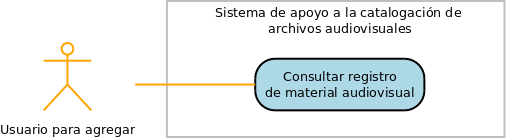
\includegraphics[width=0.8\textwidth]{CasoDeUso_Agregar_ConsultarRegistro.png}
\end{figure}

% Descripción
\textbf{Descipción: } Acción que permite mostrar la información completa de un archivo audiovisual cuya portada es mostrada en pantalla.

% Precondiciones
\textbf{Precondiciones:} Estar en alguna de las páginas que muestra los archivos audiovisuales por década.

% Flujo Normal de Eventos (tabla)
\begin{adjustwidth}{-6em}{-6em}
	\begin{center}
		\begin{tabularx}{1.2\textwidth}{ | p{0.7cm} | X | p{0.7cm} | X | p{1.5cm} | }
			\hline
			\rowcolor{NewBlue} \multicolumn{5}{|c|}{\textbf{Flujo normal de eventos}} \\
			\hline
			\multicolumn{2}{|c|}{\textbf{Actor(es)}}	&	\multicolumn{2}{c|}{\textbf{Sistema}}	&	\textbf{Alterno} \\
			\hline
			\textbf{Paso}	&	\textbf{Acción}	&	\textbf{Paso}	&	\textbf{Acción}	&	\textbf{ID} \\
			\hline
			1 & 
			Dar clic en la portada del audiovisual que se desea ver &
			2 &
			El sistema pide todos los datos del audiovisual a la base de datos &
			E1 \\
			\hline
			& 
			&
			3 &
			El sistema muestra una ventana emergente con toda la información del audiovisual. & 
			A1 \\
			\hline
		\end{tabularx}
	\end{center}
\end{adjustwidth}

% Flujo Alterno (en caso de ser necesario)
\begin{adjustwidth}{-6em}{-6em}
	\begin{center}
		\begin{tabularx}{1.2\textwidth}{ | p{0.6cm} | X | X | }
			\hline
			\rowcolor{NewBlue} \multicolumn{3}{|c|}{\textbf{Flujo alterno de eventos}} \\
			\hline
			\textbf{ID}	&	\textbf{Descripción}	&	\textbf{Acción} \\
			\hline
			A1 &
			El usuario da clic en el botón de ``Ver más'' para ver información específica del archivo audiovisual &
			El sistema muestra en la parte inferior toda la información disponible del archivo audiovisual separada por áreas. \\
			\hline
		\end{tabularx}
	\end{center}
\end{adjustwidth}

% Flujo de Excepcion de Eventos (tabla)
\begin{adjustwidth}{-6em}{-6em}
	\begin{center}
		\begin{tabularx}{1.2\textwidth}{ | p{0.6cm} | X | X | }
			\hline
			\rowcolor{NewBlue} \multicolumn{3}{|c|}{\textbf{Flujo excepcional de eventos}} \\
			\hline
			\textbf{ID}	&	\textbf{Descripción}	&	\textbf{Acción} \\
			\hline
			E1 &
			No hay conexión con la base de datos. &
			El sistema devuelve un mensaje de error de conexión. \\
			\hline
		\end{tabularx}
	\end{center}
\end{adjustwidth}

% Post-condiciones
\textbf{Postcondiciones:} El entorno de la página se oscurece para dar enfoque a la información completa del archivo audiovisual.

% Casos de prueba para flujo normal (tabla) y su prototipo (imagen)
%\begin{figure}[H]
%	\centering
%	\includegraphics[width=0.8\textwidth]{imagen.png}
%\end{figure}

\begin{adjustwidth}{-6em}{-6em}
	\begin{center}
		\begin{tabularx}{1.2\textwidth}{ | X | X | }
			\hline
			\rowcolor{NewBlue} \multicolumn{2}{|c|}{\textbf{Casos de prueba (Flujo normal)}} \\
			\hline
			\textbf{Entradas}	&	\textbf{Resultado esperado} \\
			\hline
			Clic en una portada de audiovisual. &
			Mostrar el contenido completo del archivo audiovisual seleccionado. \\
			\hline
		\end{tabularx}
	\end{center}
\end{adjustwidth}

% Casos de prueba (Flujo alterno de eventos) [cuando es necesario]

%\begin{figure}[H]
%	\centering
%	\includegraphics[width=0.8\textwidth]{imagen.png}
%\end{figure}

\begin{adjustwidth}{-6em}{-6em}
	\begin{center}
		\begin{tabularx}{1.2\textwidth}{ | p{0.6cm} | X | X | }
			\hline
			\rowcolor{NewBlue} \multicolumn{3}{|c|}{\textbf{Caso de prueba (Flujo alterno)}} \\
			\hline
			\textbf{ID}	&	\textbf{Entrada}	&	\textbf{Resultado esperado} \\
			\hline
			A1 &
			Clic en el botón de ``Ver más''. &
			El sistema muestra en la parte inferior toda la información disponible del archivo audiovisual separada por áreas. \\
			\hline
		\end{tabularx}
	\end{center}
\end{adjustwidth}

% Casos de prueba para excepción de eventos (tabla) y su prototipo (imagen)
%\begin{figure}[H]
%	\centering
%	\includegraphics[width=0.8\textwidth]{imagen.png}
%\end{figure}

\begin{adjustwidth}{-6em}{-6em}
	\begin{center}
		\begin{tabularx}{1.2\textwidth}{ | p{0.6cm} | X | X | }
			\hline
			\rowcolor{NewBlue} \multicolumn{3}{|c|}{\textbf{Caso de prueba (Flujo excepcional)}} \\
			\hline
			\textbf{ID}	&	\textbf{Entrada}	&	\textbf{Resultado esperado} \\
			\hline
			E1 &
			Clic en una portada de audiovisual. &
			El sistema devuelve un mensaje de error de conexión. \\
			\hline
		\end{tabularx}
	\end{center}
\end{adjustwidth}

\subsubsection{Realizar búsquedas de material audiovisual}
% Actor
\textbf{Actor:} Usuario para agregar

% Imagen del diagrama específico del caso
\begin{figure}[H]
	\centering
	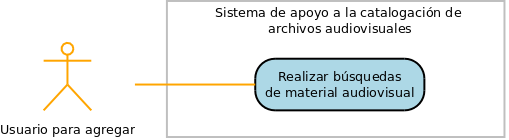
\includegraphics[width=0.8\textwidth]{CasoDeUso_Agregar_Busqueda.png}
\end{figure}

% Descripción
\textbf{Descipción: } Acción que permite realizar una búsqueda de material audiovisual.

% Precondiciones
\textbf{Precondiciones:} Estar en cualquiera de las páginas del sistema.

% Flujo Normal de Eventos (tabla)
\begin{adjustwidth}{-6em}{-6em}
	\begin{center}
		\begin{tabularx}{1.2\textwidth}{ | p{0.7cm} | X | p{0.7cm} | X | p{1.5cm} | }
			\hline
			\rowcolor{NewBlue} \multicolumn{5}{|c|}{\textbf{Flujo normal de eventos}} \\
			\hline
			\multicolumn{2}{|c|}{\textbf{Actor(es)}}	&	\multicolumn{2}{c|}{\textbf{Sistema}}	&	\textbf{Alterno} \\
			\hline
			\textbf{Paso}	&	\textbf{Acción}	&	\textbf{Paso}	&	\textbf{Acción}	&	\textbf{ID} \\
			\hline
			1 & 
			Escribir texto de búsqueda en el campo situado en la parte superior del navegador y presionar \textit{Enter} en el teclado o clic en el botón con el icono de lupa situado a la derecha &
			2 &
			El sistema realiza una búsqueda dentro de la base de datos con las coincidencias de las palabras escritas &
			E1 \\
			\hline
			& 
			&
			3 &
			El sistema muestra los resultados en pantalla utilizando la misma vista que los archivos audiovisuales por década (mostrando la portada, el título y el año) & 
			E2\\
			\hline
		\end{tabularx}
	\end{center}
\end{adjustwidth}

% Flujo de Excepcion de Eventos (tabla)
\begin{adjustwidth}{-6em}{-6em}
	\begin{center}
		\begin{tabularx}{1.2\textwidth}{ | p{0.6cm} | X | X | }
			\hline
			\rowcolor{NewBlue} \multicolumn{3}{|c|}{\textbf{Flujo excepcional de eventos}} \\
			\hline
			\textbf{ID}	&	\textbf{Descripción}	&	\textbf{Acción} \\
			\hline
			E1 &
			No hay conexión con la base de datos. &
			El sistema devuelve un mensaje de error de conexión. \\
			\hline
			E2 &
			No hay coincidencias de búsqueda en la base de datos. &
			El sistema muestra un texto indicando no hay resultados de la búsqueda. \\
			\hline
		\end{tabularx}
	\end{center}
\end{adjustwidth}

% Post-condiciones
\textbf{Postcondiciones:} El usuario es autodirigido a la página que muestra los audiovisuales resultantes de la búsqueda.

% Casos de prueba para flujo normal (tabla) y su prototipo (imagen)
%\begin{figure}[H]
%	\centering
%	\includegraphics[width=0.8\textwidth]{imagen.png}
%\end{figure}

\begin{adjustwidth}{-6em}{-6em}
	\begin{center}
		\begin{tabularx}{1.2\textwidth}{ | X | X | }
			\hline
			\rowcolor{NewBlue} \multicolumn{2}{|c|}{\textbf{Casos de prueba (Flujo normal)}} \\
			\hline
			\textbf{Entradas}	&	\textbf{Resultado esperado} \\
			\hline
			Escribir texto de búsqueda y presionar \textit{Enter} en el teclado o dar clic en el botón de búsqueda &
			El sistema muestra los audiovisuales resultantes en pantalla. \\
			\hline
		\end{tabularx}
	\end{center}
\end{adjustwidth}

% Casos de prueba para excepción de eventos (tabla) y su prototipo (imagen)
%\begin{figure}[H]
%	\centering
%	\includegraphics[width=0.8\textwidth]{imagen.png}
%\end{figure}

\begin{adjustwidth}{-6em}{-6em}
	\begin{center}
		\begin{tabularx}{1.2\textwidth}{ | p{0.6cm} | X | X | }
			\hline
			\rowcolor{NewBlue} \multicolumn{3}{|c|}{\textbf{Caso de prueba (Flujo excepcional)}} \\
			\hline
			\textbf{ID}	&	\textbf{Entrada}	&	\textbf{Resultado esperado} \\
			\hline
			E1 &
			No hay conexión con la base de datos. &
			El sistema devuelve un mensaje de error de conexión. \\
			\hline
			E2 &
			No hay coincidencias de búsqueda en la base de datos. &
			El sistema muestra un texto indicando no hay resultados de la búsqueda. \\
			\hline
		\end{tabularx}
	\end{center}
\end{adjustwidth}

\subsubsection{Agregar nuevo registro de material audiovisual}
% Actor
\textbf{Actor:} Usuario para agregar

% Imagen del diagrama específico del caso
\begin{figure}[H]
	\centering
	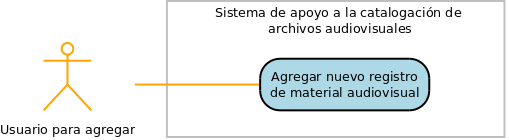
\includegraphics[width=0.8\textwidth]{CasoDeUso_Agregar_AgregarNuevoRegistro.png}
\end{figure}

% Descripción
\textbf{Descipción: } Acción que permite al usuario agregar un nuevo archivo audiovisual al sistema.

% Precondiciones
\textbf{Precondiciones:} Tener iniciada la sesion del usuario y tener los datos de los campos necesarios para agregar el nuevo archivo audiovisual.

% Flujo Normal de Eventos (tabla)
\begin{adjustwidth}{-6em}{-6em}
	\begin{center}
		\begin{tabularx}{1.2\textwidth}{ | p{0.7cm} | X | p{0.7cm} | X | p{1.5cm} | }
			\hline
			\rowcolor{NewBlue} \multicolumn{5}{|c|}{\textbf{Flujo normal de eventos}} \\
			\hline
			\multicolumn{2}{|c|}{\textbf{Actor(es)}}	&	\multicolumn{2}{c|}{\textbf{Sistema}}	&	\textbf{Alterno} \\
			\hline
			\textbf{Paso}	&	\textbf{Acción}	&	\textbf{Paso}	&	\textbf{Acción}	&	\textbf{ID} \\
			\hline
			1 & 
			 El usuario ya estando es sesión da clic en la pestaña audiovisual.&
			2 &
			El sistema mostrará una página donde contendrá las portadas de las décadas junto con un botón de agregar.&
			E1
			\\
			\hline
			3 & 
			 El usuario da clic en el botón de agregar.&
			4 &
			El sistema mostrará una pagína donde contendrá los formularios para que el usuario escriba la nueva información del archivo a agregar&
			\\
			\hline
			5 & 
			 El usuario llenará los campos con la información solicitada en el formulario y despueś dará clic en agregar.&
			6 &
			El sistema mostrará un mensaje de éxito y redirigirá a la pestaña audiovidual y mostrará el nuevo elemento agregado.&
			E1,E2,A1
			\\
			\hline
		\end{tabularx}
	\end{center}
\end{adjustwidth}

% Flujo Alterno (en caso de ser necesario)
\begin{adjustwidth}{-6em}{-6em}
	\begin{center}
		\begin{tabularx}{1.2\textwidth}{ | p{0.6cm} | X | X | }
			\hline
			\rowcolor{NewBlue} \multicolumn{3}{|c|}{\textbf{Flujo alterno de eventos}} \\
			\hline
			\textbf{ID}	&	\textbf{Descripción}	&	\textbf{Acción} \\
			\hline
			A1 &
			El usuario da clic en una década específica y se mostrará junto a las portadas de los archivos el botón de agregar donde, al darle clic aparecerá el mismo formulario para agregar pero con la diferencia de que el archivo solo se agregará para la década específica seleccionada.&
			El sistema mostrará un mensaje de éxito y  autoredirige al usuario a la página donde estan todas las portadas de los archivos audiovisuales de la década con el nuevo registro. \\
			\hline
		\end{tabularx}
	\end{center}
\end{adjustwidth}

% Flujo de Excepcion de Eventos (tabla)
\begin{adjustwidth}{-6em}{-6em}
	\begin{center}
		\begin{tabularx}{1.2\textwidth}{ | p{0.6cm} | X | X | }
			\hline
			\rowcolor{NewBlue} \multicolumn{3}{|c|}{\textbf{Flujo excepcional de eventos}} \\
			\hline
			\textbf{ID}	&	\textbf{Descripción}	&	\textbf{Acción} \\
			\hline
			E1 &
			No hay conexión con la base de datos. &
			El sistema devuelve un mensaje de error de conexión. \\
			\hline
			E2 &
			Los campos del usuario no estan llenados correctamente. &
			El sistema muestra un mensaje error por cada campo incorrecto y desactiva el botón de agregar. \\
			\hline
		\end{tabularx}
	\end{center}
\end{adjustwidth}

% Post-condiciones
\textbf{Postcondiciones:} El usuario es autodirigido a la página que muestra el nuevo archivo audiovisual agregado

% Casos de prueba para flujo normal (tabla) y su prototipo (imagen)
%\begin{figure}[H]
%	\centering
%	\includegraphics[width=0.8\textwidth]{imagen.png}
%\end{figure}

\begin{adjustwidth}{-6em}{-6em}
	\begin{center}
		\begin{tabularx}{1.2\textwidth}{ | X | X | }
			\hline
			\rowcolor{NewBlue} \multicolumn{2}{|c|}{\textbf{Casos de prueba (Flujo normal)}} \\
			\hline
			\textbf{Entradas}	&	\textbf{Resultado esperado} \\
			\hline
			Ir a la pestaña de audiovisuales. &
			El sistema muestra las portadas de las décadas en pantalla junto con el boton de agregar. \\
			\hline
			Dar clic en el botón de agregar.&
			El sistema muestrá el formulario con sus respectivos campos a llenar en pantalla. \\
			\hline
			El usuario inserta la información en los campos necesarios del nuevo archivo audiovisual y da clic en agregar.&
			El sistema manda un mensaje de que se ha agregado con exíto el archivo audiovisual.\\
			\hline
		\end{tabularx}
	\end{center}
\end{adjustwidth}

% Casos de prueba (Flujo alterno de eventos) [cuando es necesario]

%\begin{figure}[H]
%	\centering
%	\includegraphics[width=0.8\textwidth]{imagen.png}
%\end{figure}

\begin{adjustwidth}{-6em}{-6em}
	\begin{center}
		\begin{tabularx}{1.2\textwidth}{ | p{0.6cm} | X | X | }
			\hline
			\rowcolor{NewBlue} \multicolumn{3}{|c|}{\textbf{Caso de prueba (Flujo alterno)}} \\
			\hline
			\textbf{ID}	&	\textbf{Entrada}	&	\textbf{Resultado esperado} \\
			\hline
			A1 &
			El usuario da clic en una década específica, se muestrá en pantalla las postadas de los archivos audiovisuales a esa década junto con el botón de agregar, da clic en el botón de agregar, se muestra el formulario inserta los datos del nuevo archivo audiovisual y da clic en el botón de agregar. &
			El sistema mostrará un mensaje de éxito y redirigirá a la página de las portadas de la década seleccionada con el nuevo archivo agregado. \\
			\hline
		\end{tabularx}
	\end{center}
\end{adjustwidth}

% Casos de prueba para excepción de eventos (tabla) y su prototipo (imagen)
%\begin{figure}[H]
%	\centering
%	\includegraphics[width=0.8\textwidth]{imagen.png}
%\end{figure}

\begin{adjustwidth}{-6em}{-6em}
	\begin{center}
		\begin{tabularx}{1.2\textwidth}{ | p{0.6cm} | X | X | }
			\hline
			\rowcolor{NewBlue} \multicolumn{3}{|c|}{\textbf{Caso de prueba (Flujo excepcional)}} \\
			\hline
			\textbf{ID}	&	\textbf{Entrada}	&	\textbf{Resultado esperado} \\
			\hline
			E1 &
			No hay conexión con la base de datos. &
			El sistema devuelve un mensaje de error de conexión. \\
			\hline
			E2 &
			Los datos insertados en los campos del formulario no son correctos. &
			El sistema muestra un mensaje de error por cada campo incorrecto y desactiva el botón de agregar. \\
			\hline
		\end{tabularx}
	\end{center}
\end{adjustwidth}

\subsubsection{Iniciar sesion como usuario de LAIS}
% Actor
\textbf{Actor:} Usuario para agregar

% Imagen del diagrama específico del caso
\begin{figure}[H]
	\centering
	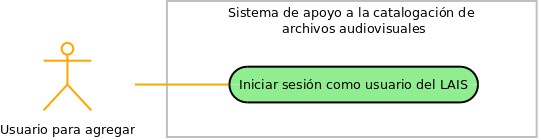
\includegraphics[width=0.8\textwidth]{CasoDeUso_Agregar_IniciarSesion.png}
\end{figure}

% Descripción
\textbf{Descipción: } Acción que permite iniciar sesión del sistema.

% Precondiciones
\textbf{Precondiciones:} Estar en cualquiera de las páginas del sistema y estar en sesión cerrada.

% Flujo Normal de Eventos (tabla)
\begin{adjustwidth}{-6em}{-6em}
	\begin{center}
		\begin{tabularx}{1.2\textwidth}{ | p{0.7cm} | X | p{0.7cm} | X | p{1.5cm} | }
			\hline
			\rowcolor{NewBlue} \multicolumn{5}{|c|}{\textbf{Flujo normal de eventos}} \\
			\hline
			\multicolumn{2}{|c|}{\textbf{Actor(es)}}	&	\multicolumn{2}{c|}{\textbf{Sistema}}	&	\textbf{Alterno} \\
			\hline
			\textbf{Paso}	&	\textbf{Acción}	&	\textbf{Paso}	&	\textbf{Acción}	&	\textbf{ID} \\
			\hline
			1 & 
			Dar clic en el botón de iniciar sesión situado en la parte superior del navegador.&
			2 &
			El sistema muestra una ventana que contiene los campos de nombre de usuario y contraseña.&\\
			\hline			
			3&
			Usuario inserta los datos correspondientes a su nombre de usuario y contraseña y da clic a iniciar sesion.&
			4&
			El sistema inicia sesión con el usuario correspondiente eliminando la ventana de iniciar sesión&
			E1,E2
			\\
			\hline
		\end{tabularx}
	\end{center}
\end{adjustwidth}

% Post-condiciones
\textbf{Postcondiciones:} El sistema cierra sesión y autoredirige al usuario a la página de inicio.

% Casos de prueba para flujo normal (tabla) y su prototipo (imagen)
%\begin{figure}[H]
%	\centering
%	\includegraphics[width=0.8\textwidth]{imagen.png}
%\end{figure}

\begin{adjustwidth}{-6em}{-6em}
	\begin{center}
		\begin{tabularx}{1.2\textwidth}{ | X | X | }
			\hline
			\rowcolor{NewBlue} \multicolumn{2}{|c|}{\textbf{Casos de prueba (Flujo normal)}} \\
			\hline
			\textbf{Entradas}	&	\textbf{Resultado esperado} \\
			\hline
			Clic en el botón de iniciar sesión. &
			El sistema muestra laa ventana de iniciar sesión. \\
			\hline
			El usuario inserta los datos correspondientes a nombre de usuario y contraseña y da clic en iniciar sesión. &
			El sistema inicia sesion con el usuario correspondiente. \\
			\hline
		\end{tabularx}
	\end{center}
\end{adjustwidth}


% Casos de prueba para excepción de eventos (tabla) y su prototipo (imagen)
%\begin{figure}[H]
%	\centering
%	\includegraphics[width=0.8\textwidth]{imagen.png}
%\end{figure}

\begin{adjustwidth}{-6em}{-6em}
	\begin{center}
		\begin{tabularx}{1.2\textwidth}{ | p{0.6cm} | X | X | }
			\hline
			\rowcolor{NewBlue} \multicolumn{3}{|c|}{\textbf{Caso de prueba (Flujo excepcional)}} \\
			\hline
			\textbf{ID}	&	\textbf{Entrada}	&	\textbf{Resultado esperado} \\
			\hline
			E1 &
			Los datos de iniciar sesión como contraseña o nombre de usuario o ambos son incorrectos. &
			El sistema devuelve un mensaje de error de los campos incorrectos. \\
			\hline
			E2 &
			No hay conexión con la base de datos. &
			El sistema devuelve un mensaje de error de conexión. \\
			\hline
		\end{tabularx}
	\end{center}
\end{adjustwidth}

\subsubsection{Cerrar sesion como usuario del LAIS}
% Actor
\textbf{Actor:} Usuario para agregar

% Imagen del diagrama específico del caso
\begin{figure}[H]
	\centering
	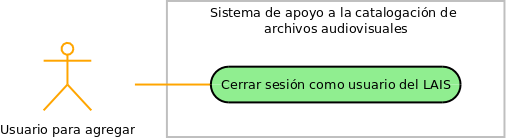
\includegraphics[width=0.8\textwidth]{CasoDeUso_Agregar_CerrarSesion.png}
\end{figure}

% Descripción
\textbf{Descipción: } Acción que permite cerrar sesión del sistema.

% Precondiciones
\textbf{Precondiciones:} Tener iniciada la sesión del usuario y estar en cualquiera de las páginas del sistema.

% Flujo Normal de Eventos (tabla)
\begin{adjustwidth}{-6em}{-6em}
	\begin{center}
		\begin{tabularx}{1.2\textwidth}{ | p{0.7cm} | X | p{0.7cm} | X | p{1.5cm} | }
			\hline
			\rowcolor{NewBlue} \multicolumn{5}{|c|}{\textbf{Flujo normal de eventos}} \\
			\hline
			\multicolumn{2}{|c|}{\textbf{Actor(es)}}	&	\multicolumn{2}{c|}{\textbf{Sistema}}	&	\textbf{Alterno} \\
			\hline
			\textbf{Paso}	&	\textbf{Acción}	&	\textbf{Paso}	&	\textbf{Acción}	&	\textbf{ID} \\
			\hline
			1 & 
			Dar clic en el botón de cerrar sesión situado en la parte superior del navegador.&
			2 &
			El sistema cierra sesión redirigiendo a la página de inicio.&			
			\\
			\hline
		\end{tabularx}
	\end{center}
\end{adjustwidth}

% Post-condiciones
\textbf{Postcondiciones:} El sistema cierra sesión y autoredirige al usuario a la página de inicio.

% Casos de prueba para flujo normal (tabla) y su prototipo (imagen)
%\begin{figure}[H]
%	\centering
%	\includegraphics[width=0.8\textwidth]{imagen.png}
%\end{figure}

\begin{adjustwidth}{-6em}{-6em}
	\begin{center}
		\begin{tabularx}{1.2\textwidth}{ | X | X | }
			\hline
			\rowcolor{NewBlue} \multicolumn{2}{|c|}{\textbf{Casos de prueba (Flujo normal)}} \\
			\hline
			\textbf{Entradas}	&	\textbf{Resultado esperado} \\
			\hline
			Clic en el botón de cerrar sesión. &
			El sistema cierra sesión. \\
			\hline
		\end{tabularx}
	\end{center}
\end{adjustwidth}

% Casos de prueba (Flujo alterno de eventos) [cuando es necesario]

%\begin{figure}[H]
%	\centering
%	\includegraphics[width=0.8\textwidth]{imagen.png}
%\end{figure}

\begin{adjustwidth}{-6em}{-6em}
	\begin{center}
		\begin{tabularx}{1.2\textwidth}{ | p{0.6cm} | X | X | }
			\hline
			\rowcolor{NewBlue} \multicolumn{3}{|c|}{\textbf{Caso de prueba (Flujo alterno)}} \\
			\hline
			\textbf{ID}	&	\textbf{Entrada}	&	\textbf{Resultado esperado} \\
			\hline
			A1 &
			Se selleciona la opción de cancelar. &
			El sistema cancela la eliminación redirigiendo a la página donde se esta consultando el archivo audiovisual. \\
			\hline
		\end{tabularx}
	\end{center}
\end{adjustwidth}

% Casos de prueba para excepción de eventos (tabla) y su prototipo (imagen)
%\begin{figure}[H]
%	\centering
%	\includegraphics[width=0.8\textwidth]{imagen.png}
%\end{figure}

\begin{adjustwidth}{-6em}{-6em}
	\begin{center}
		\begin{tabularx}{1.2\textwidth}{ | p{0.6cm} | X | X | }
			\hline
			\rowcolor{NewBlue} \multicolumn{3}{|c|}{\textbf{Caso de prueba (Flujo excepcional)}} \\
			\hline
			\textbf{ID}	&	\textbf{Entrada}	&	\textbf{Resultado esperado} \\
			\hline
			E1 &
			No hay conexión con la base de datos. &
			El sistema devuelve un mensaje de error de conexión. \\
			\hline
		\end{tabularx}
	\end{center}
\end{adjustwidth}

\subsection{Usuario administrador}

\subsubsection{Consultar registro de material audiovisual}
% Actor
\textbf{Actor:} Usuario administrador

% Imagen del diagrama específico del caso
\begin{figure}[H]
	\centering
	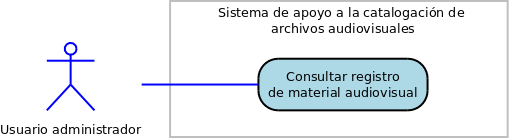
\includegraphics[width=0.8\textwidth]{CasoDeUso_Administrador_ConsultarRegistro.png}
\end{figure}

% Descripción
\textbf{Descipción: } Acción que permite mostrar la información completa de un archivo audiovisual cuya portada es mostrada en pantalla.

% Precondiciones
\textbf{Precondiciones:} Estar en alguna de las páginas que muestra los archivos audiovisuales por década.

% Flujo Normal de Eventos (tabla)
\begin{adjustwidth}{-6em}{-6em}
	\begin{center}
		\begin{tabularx}{1.2\textwidth}{ | p{0.7cm} | X | p{0.7cm} | X | p{1.5cm} | }
			\hline
			\rowcolor{NewBlue} \multicolumn{5}{|c|}{\textbf{Flujo normal de eventos}} \\
			\hline
			\multicolumn{2}{|c|}{\textbf{Actor(es)}}	&	\multicolumn{2}{c|}{\textbf{Sistema}}	&	\textbf{Alterno} \\
			\hline
			\textbf{Paso}	&	\textbf{Acción}	&	\textbf{Paso}	&	\textbf{Acción}	&	\textbf{ID} \\
			\hline
			1 & 
			Dar clic en la portada del audiovisual que se desea ver &
			2 &
			El sistema pide todos los datos del audiovisual a la base de datos &
			E1 \\
			\hline
			& 
			&
			3 &
			El sistema muestra una ventana emergente con toda la información del audiovisual. & 
			A1 \\
			\hline
		\end{tabularx}
	\end{center}
\end{adjustwidth}

% Flujo Alterno (en caso de ser necesario)
\begin{adjustwidth}{-6em}{-6em}
	\begin{center}
		\begin{tabularx}{1.2\textwidth}{ | p{0.6cm} | X | X | }
			\hline
			\rowcolor{NewBlue} \multicolumn{3}{|c|}{\textbf{Flujo alterno de eventos}} \\
			\hline
			\textbf{ID}	&	\textbf{Descripción}	&	\textbf{Acción} \\
			\hline
			A1 &
			El usuario da clic en el botón de ``Ver más'' para ver información específica del archivo audiovisual &
			El sistema muestra en la parte inferior toda la información disponible del archivo audiovisual separada por áreas. \\
			\hline
		\end{tabularx}
	\end{center}
\end{adjustwidth}

% Flujo de Excepcion de Eventos (tabla)
\begin{adjustwidth}{-6em}{-6em}
	\begin{center}
		\begin{tabularx}{1.2\textwidth}{ | p{0.6cm} | X | X | }
			\hline
			\rowcolor{NewBlue} \multicolumn{3}{|c|}{\textbf{Flujo excepcional de eventos}} \\
			\hline
			\textbf{ID}	&	\textbf{Descripción}	&	\textbf{Acción} \\
			\hline
			E1 &
			No hay conexión con la base de datos. &
			El sistema devuelve un mensaje de error de conexión. \\
			\hline
		\end{tabularx}
	\end{center}
\end{adjustwidth}

% Post-condiciones
\textbf{Postcondiciones:} El entorno de la página se oscurece para dar enfoque a la información completa del archivo audiovisual.

% Casos de prueba para flujo normal (tabla) y su prototipo (imagen)
%\begin{figure}[H]
%	\centering
%	\includegraphics[width=0.8\textwidth]{imagen.png}
%\end{figure}

\begin{adjustwidth}{-6em}{-6em}
	\begin{center}
		\begin{tabularx}{1.2\textwidth}{ | X | X | }
			\hline
			\rowcolor{NewBlue} \multicolumn{2}{|c|}{\textbf{Casos de prueba (Flujo normal)}} \\
			\hline
			\textbf{Entradas}	&	\textbf{Resultado esperado} \\
			\hline
			Clic en una portada de audiovisual. &
			Mostrar el contenido completo del archivo audiovisual seleccionado. \\
			\hline
		\end{tabularx}
	\end{center}
\end{adjustwidth}

% Casos de prueba (Flujo alterno de eventos) [cuando es necesario]

%\begin{figure}[H]
%	\centering
%	\includegraphics[width=0.8\textwidth]{imagen.png}
%\end{figure}

\begin{adjustwidth}{-6em}{-6em}
	\begin{center}
		\begin{tabularx}{1.2\textwidth}{ | p{0.6cm} | X | X | }
			\hline
			\rowcolor{NewBlue} \multicolumn{3}{|c|}{\textbf{Caso de prueba (Flujo alterno)}} \\
			\hline
			\textbf{ID}	&	\textbf{Entrada}	&	\textbf{Resultado esperado} \\
			\hline
			A1 &
			Clic en el botón de ``Ver más''. &
			El sistema muestra en la parte inferior toda la información disponible del archivo audiovisual separada por áreas. \\
			\hline
		\end{tabularx}
	\end{center}
\end{adjustwidth}

% Casos de prueba para excepción de eventos (tabla) y su prototipo (imagen)
%\begin{figure}[H]
%	\centering
%	\includegraphics[width=0.8\textwidth]{imagen.png}
%\end{figure}

\begin{adjustwidth}{-6em}{-6em}
	\begin{center}
		\begin{tabularx}{1.2\textwidth}{ | p{0.6cm} | X | X | }
			\hline
			\rowcolor{NewBlue} \multicolumn{3}{|c|}{\textbf{Caso de prueba (Flujo excepcional)}} \\
			\hline
			\textbf{ID}	&	\textbf{Entrada}	&	\textbf{Resultado esperado} \\
			\hline
			E1 &
			Clic en una portada de audiovisual. &
			El sistema devuelve un mensaje de error de conexión. \\
			\hline
		\end{tabularx}
	\end{center}
\end{adjustwidth}

\subsubsection{Realizar búsquedas de material audiovisual}
% Actor
\textbf{Actor:} Usuario administrador

% Imagen del diagrama específico del caso
\begin{figure}[H]
	\centering
	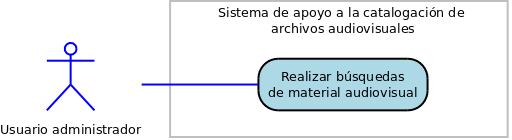
\includegraphics[width=0.8\textwidth]{CasoDeUso_Administrador_Busqueda.png}
\end{figure}

% Descripción
\textbf{Descipción: } Acción que permite realizar una búsqueda de material audiovisual.

% Precondiciones
\textbf{Precondiciones:} Estar en cualquiera de las páginas del sistema.

% Flujo Normal de Eventos (tabla)
\begin{adjustwidth}{-6em}{-6em}
	\begin{center}
		\begin{tabularx}{1.2\textwidth}{ | p{0.7cm} | X | p{0.7cm} | X | p{1.5cm} | }
			\hline
			\rowcolor{NewBlue} \multicolumn{5}{|c|}{\textbf{Flujo normal de eventos}} \\
			\hline
			\multicolumn{2}{|c|}{\textbf{Actor(es)}}	&	\multicolumn{2}{c|}{\textbf{Sistema}}	&	\textbf{Alterno} \\
			\hline
			\textbf{Paso}	&	\textbf{Acción}	&	\textbf{Paso}	&	\textbf{Acción}	&	\textbf{ID} \\
			\hline
			1 & 
			Escribir texto de búsqueda en el campo situado en la parte superior del navegador y presionar \textit{Enter} en el teclado o clic en el botón con el icono de lupa situado a la derecha &
			2 &
			El sistema realiza una búsqueda dentro de la base de datos con las coincidencias de las palabras escritas &
			E1 \\
			\hline
			& 
			&
			3 &
			El sistema muestra los resultados en pantalla utilizando la misma vista que los archivos audiovisuales por década (mostrando la portada, el título y el año) & 
			E2\\
			\hline
		\end{tabularx}
	\end{center}
\end{adjustwidth}

% Flujo de Excepcion de Eventos (tabla)
\begin{adjustwidth}{-6em}{-6em}
	\begin{center}
		\begin{tabularx}{1.2\textwidth}{ | p{0.6cm} | X | X | }
			\hline
			\rowcolor{NewBlue} \multicolumn{3}{|c|}{\textbf{Flujo excepcional de eventos}} \\
			\hline
			\textbf{ID}	&	\textbf{Descripción}	&	\textbf{Acción} \\
			\hline
			E1 &
			No hay conexión con la base de datos. &
			El sistema devuelve un mensaje de error de conexión. \\
			\hline
			E2 &
			No hay coincidencias de búsqueda en la base de datos. &
			El sistema muestra un texto indicando no hay resultados de la búsqueda. \\
			\hline
		\end{tabularx}
	\end{center}
\end{adjustwidth}

% Post-condiciones
\textbf{Postcondiciones:} El usuario es autodirigido a la página que muestra los audiovisuales resultantes de la búsqueda.

% Casos de prueba para flujo normal (tabla) y su prototipo (imagen)
%\begin{figure}[H]
%	\centering
%	\includegraphics[width=0.8\textwidth]{imagen.png}
%\end{figure}

\begin{adjustwidth}{-6em}{-6em}
	\begin{center}
		\begin{tabularx}{1.2\textwidth}{ | X | X | }
			\hline
			\rowcolor{NewBlue} \multicolumn{2}{|c|}{\textbf{Casos de prueba (Flujo normal)}} \\
			\hline
			\textbf{Entradas}	&	\textbf{Resultado esperado} \\
			\hline
			Escribir texto de búsqueda y presionar \textit{Enter} en el teclado o dar clic en el botón de búsqueda &
			El sistema muestra los audiovisuales resultantes en pantalla. \\
			\hline
		\end{tabularx}
	\end{center}
\end{adjustwidth}

% Casos de prueba para excepción de eventos (tabla) y su prototipo (imagen)
%\begin{figure}[H]
%	\centering
%	\includegraphics[width=0.8\textwidth]{imagen.png}
%\end{figure}

\begin{adjustwidth}{-6em}{-6em}
	\begin{center}
		\begin{tabularx}{1.2\textwidth}{ | p{0.6cm} | X | X | }
			\hline
			\rowcolor{NewBlue} \multicolumn{3}{|c|}{\textbf{Caso de prueba (Flujo excepcional)}} \\
			\hline
			\textbf{ID}	&	\textbf{Entrada}	&	\textbf{Resultado esperado} \\
			\hline
			E1 &
			No hay conexión con la base de datos. &
			El sistema devuelve un mensaje de error de conexión. \\
			\hline
			E2 &
			No hay coincidencias de búsqueda en la base de datos. &
			El sistema muestra un texto indicando no hay resultados de la búsqueda. \\
			\hline
		\end{tabularx}
	\end{center}
\end{adjustwidth}

\subsubsection{Agregar nuevo registro de material audiovisual}
% Actor
\textbf{Actor:} Usuario administrador

% Imagen del diagrama específico del caso
\begin{figure}[H]
	\centering
	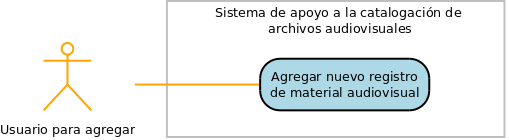
\includegraphics[width=0.8\textwidth]{CasoDeUso_Agregar_AgregarNuevoRegistro.png}
\end{figure}

% Descripción
\textbf{Descipción: } Acción que permite al usuario agregar un nuevo archivo audiovisual al sistema.

% Precondiciones
\textbf{Precondiciones:} Tener iniciada la sesion del usuario y tener los datos de los campos necesarios para agregar el nuevo archivo audiovisual.

% Flujo Normal de Eventos (tabla)
\begin{adjustwidth}{-6em}{-6em}
	\begin{center}
		\begin{tabularx}{1.2\textwidth}{ | p{0.7cm} | X | p{0.7cm} | X | p{1.5cm} | }
			\hline
			\rowcolor{NewBlue} \multicolumn{5}{|c|}{\textbf{Flujo normal de eventos}} \\
			\hline
			\multicolumn{2}{|c|}{\textbf{Actor(es)}}	&	\multicolumn{2}{c|}{\textbf{Sistema}}	&	\textbf{Alterno} \\
			\hline
			\textbf{Paso}	&	\textbf{Acción}	&	\textbf{Paso}	&	\textbf{Acción}	&	\textbf{ID} \\
			\hline
			1 & 
			 El usuario ya estando es sesión da clic en la pestaña audiovisual.&
			2 &
			El sistema mostrará una página donde contendrá las portadas de las décadas junto con un botón de agregar.&
			E1
			\\
			\hline
			3 & 
			 El usuario da clic en el botón de agregar.&
			4 &
			El sistema mostrará una pagína donde contendrá los formularios para que el usuario escriba la nueva información del archivo a agregar&
			\\
			\hline
			5 & 
			 El usuario llenará los campos con la información solicitada en el formulario y despueś dará clic en agregar.&
			6 &
			El sistema mostrará un mensaje de éxito y redirigirá a la pestaña audiovidual y mostrará el nuevo elemento agregado.&
			E1,E2,A1
			\\
			\hline
		\end{tabularx}
	\end{center}
\end{adjustwidth}

% Flujo Alterno (en caso de ser necesario)
\begin{adjustwidth}{-6em}{-6em}
	\begin{center}
		\begin{tabularx}{1.2\textwidth}{ | p{0.6cm} | X | X | }
			\hline
			\rowcolor{NewBlue} \multicolumn{3}{|c|}{\textbf{Flujo alterno de eventos}} \\
			\hline
			\textbf{ID}	&	\textbf{Descripción}	&	\textbf{Acción} \\
			\hline
			A1 &
			El usuario da clic en una década específica y se mostrará junto a las portadas de los archivos el botón de agregar donde, al darle clic aparecerá el mismo formulario para agregar pero con la diferencia de que el archivo solo se agregará para la década específica seleccionada.&
			El sistema mostrará un mensaje de éxito y  autoredirige al usuario a la página donde estan todas las portadas de los archivos audiovisuales de la década con el nuevo registro. \\
			\hline
		\end{tabularx}
	\end{center}
\end{adjustwidth}

% Flujo de Excepcion de Eventos (tabla)
\begin{adjustwidth}{-6em}{-6em}
	\begin{center}
		\begin{tabularx}{1.2\textwidth}{ | p{0.6cm} | X | X | }
			\hline
			\rowcolor{NewBlue} \multicolumn{3}{|c|}{\textbf{Flujo excepcional de eventos}} \\
			\hline
			\textbf{ID}	&	\textbf{Descripción}	&	\textbf{Acción} \\
			\hline
			E1 &
			No hay conexión con la base de datos. &
			El sistema devuelve un mensaje de error de conexión. \\
			\hline
			E2 &
			Los campos del usuario no estan llenados correctamente. &
			El sistema muestra un mensaje error por cada campo incorrecto y desactiva el botón de agregar. \\
			\hline
		\end{tabularx}
	\end{center}
\end{adjustwidth}

% Post-condiciones
\textbf{Postcondiciones:} El usuario es autodirigido a la página que muestra el nuevo archivo audiovisual agregado

% Casos de prueba para flujo normal (tabla) y su prototipo (imagen)
%\begin{figure}[H]
%	\centering
%	\includegraphics[width=0.8\textwidth]{imagen.png}
%\end{figure}

\begin{adjustwidth}{-6em}{-6em}
	\begin{center}
		\begin{tabularx}{1.2\textwidth}{ | X | X | }
			\hline
			\rowcolor{NewBlue} \multicolumn{2}{|c|}{\textbf{Casos de prueba (Flujo normal)}} \\
			\hline
			\textbf{Entradas}	&	\textbf{Resultado esperado} \\
			\hline
			Ir a la pestaña de audiovisuales. &
			El sistema muestra las portadas de las décadas en pantalla junto con el boton de agregar. \\
			\hline
			Dar clic en el botón de agregar.&
			El sistema muestrá el formulario con sus respectivos campos a llenar en pantalla. \\
			\hline
			El usuario inserta la información en los campos necesarios del nuevo archivo audiovisual y da clic en agregar.&
			El sistema manda un mensaje de que se ha agregado con exíto el archivo audiovisual.\\
			\hline
		\end{tabularx}
	\end{center}
\end{adjustwidth}

% Casos de prueba (Flujo alterno de eventos) [cuando es necesario]

%\begin{figure}[H]
%	\centering
%	\includegraphics[width=0.8\textwidth]{imagen.png}
%\end{figure}

\begin{adjustwidth}{-6em}{-6em}
	\begin{center}
		\begin{tabularx}{1.2\textwidth}{ | p{0.6cm} | X | X | }
			\hline
			\rowcolor{NewBlue} \multicolumn{3}{|c|}{\textbf{Caso de prueba (Flujo alterno)}} \\
			\hline
			\textbf{ID}	&	\textbf{Entrada}	&	\textbf{Resultado esperado} \\
			\hline
			A1 &
			El usuario da clic en una década específica, se muestrá en pantalla las postadas de los archivos audiovisuales a esa década junto con el botón de agregar, da clic en el botón de agregar, se muestra el formulario inserta los datos del nuevo archivo audiovisual y da clic en el botón de agregar. &
			El sistema mostrará un mensaje de éxito y redirigirá a la página de las portadas de la década seleccionada con el nuevo archivo agregado. \\
			\hline
		\end{tabularx}
	\end{center}
\end{adjustwidth}

% Casos de prueba para excepción de eventos (tabla) y su prototipo (imagen)
%\begin{figure}[H]
%	\centering
%	\includegraphics[width=0.8\textwidth]{imagen.png}
%\end{figure}

\begin{adjustwidth}{-6em}{-6em}
	\begin{center}
		\begin{tabularx}{1.2\textwidth}{ | p{0.6cm} | X | X | }
			\hline
			\rowcolor{NewBlue} \multicolumn{3}{|c|}{\textbf{Caso de prueba (Flujo excepcional)}} \\
			\hline
			\textbf{ID}	&	\textbf{Entrada}	&	\textbf{Resultado esperado} \\
			\hline
			E1 &
			No hay conexión con la base de datos. &
			El sistema devuelve un mensaje de error de conexión. \\
			\hline
			E2 &
			Los datos insertados en los campos del formulario no son correctos. &
			El sistema muestra un mensaje de error por cada campo incorrecto y desactiva el botón de agregar. \\
			\hline
		\end{tabularx}
	\end{center}
\end{adjustwidth}

\subsubsection{Editar registro existente de material audiovisual}
% Actor
\textbf{Actor:} Usuario administrador

% Imagen del diagrama específico del caso
\begin{figure}[H]
	\centering
	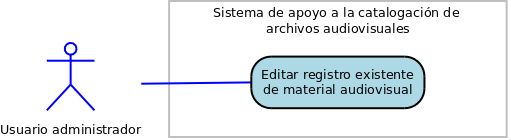
\includegraphics[width=0.8\textwidth]{CasoDeUso_Administrador_EditarRegistro.png}
\end{figure}

% Descripción
\textbf{Descipción: } Acción que permite a un usuario editar un registro.

% Precondiciones
\textbf{Precondiciones:} Tener iniciada la sesion del usuario y haber consultado el registro audiovisual que se desea editar.

% Flujo Normal de Eventos (tabla)
\begin{adjustwidth}{-6em}{-6em}
	\begin{center}
		\begin{tabularx}{1.2\textwidth}{ | p{0.7cm} | X | p{0.7cm} | X | p{1.5cm} | }
			\hline
			\rowcolor{NewBlue} \multicolumn{5}{|c|}{\textbf{Flujo normal de eventos}} \\
			\hline
			\multicolumn{2}{|c|}{\textbf{Actor(es)}}	&	\multicolumn{2}{c|}{\textbf{Sistema}}	&	\textbf{Alterno} \\
			\hline
			\textbf{Paso}	&	\textbf{Acción}	&	\textbf{Paso}	&	\textbf{Acción}	&	\textbf{ID} \\
			\hline
			1 & 
			Con sesión iniciada y consultando el registro que se desea editar, dar clic en el botón de edición.&
			2 &
			El sistema redirige a una nueva página con un formulario pre--llenado con la información existente del registo.&
			E1			
			\\
			\hline
			3
			&
			El usuario cambia, elimina o agrega información en los campos del formulario y da clic en el botón de \textit{Enviar}.
			&
			4 &
			El sistema envia la información y actualiza la base de datos mostrando un mensaje éxito en la edición. Redirige al usuario a la página de \textit{Décadas}.& 
			A1, E1, E2 \\
			\hline
		\end{tabularx}
	\end{center}
\end{adjustwidth}

% Flujo Alterno (en caso de ser necesario)
\begin{adjustwidth}{-6em}{-6em}
	\begin{center}
		\begin{tabularx}{1.2\textwidth}{ | p{0.6cm} | X | X | }
			\hline
			\rowcolor{NewBlue} \multicolumn{3}{|c|}{\textbf{Flujo alterno de eventos}} \\
			\hline
			\textbf{ID}	&	\textbf{Descripción}	&	\textbf{Acción} \\
			\hline
			A1 &
			El usuario selecciona el botón de cancelar la edición del registro &
			El sistema cancela la edición y el envio de información redirigiendo al usuario a la página anterior.\\
			\hline
		\end{tabularx}
	\end{center}
\end{adjustwidth}

% Flujo de Excepcion de Eventos (tabla)
\begin{adjustwidth}{-6em}{-6em}
	\begin{center}
		\begin{tabularx}{1.2\textwidth}{ | p{0.6cm} | X | X | }
			\hline
			\rowcolor{NewBlue} \multicolumn{3}{|c|}{\textbf{Flujo excepcional de eventos}} \\
			\hline
			\textbf{ID}	&	\textbf{Descripción}	&	\textbf{Acción} \\
			\hline
			E1 &
			No hay conexión con la base de datos. &
			El sistema devuelve un mensaje de error de conexión. \\
			\hline
			E2 &
			Los datos insertados en los campos del formulario no son correctos. &
			El sistema muestra un mensaje de error por cada campo incorrecto y desactiva el botón de agregar. \\
			\hline
		\end{tabularx}
	\end{center}
\end{adjustwidth}

% Post-condiciones
\textbf{Postcondiciones:} La base de datos queda actualizada con los cambios realizados. Dichos cambios se reflejarán inmediatamente en el sistema si se consulta el mismo registro.

% Casos de prueba para flujo normal (tabla) y su prototipo (imagen)
%\begin{figure}[H]
%	\centering
%	\includegraphics[width=0.8\textwidth]{imagen.png}
%\end{figure}

\begin{adjustwidth}{-6em}{-6em}
	\begin{center}
		\begin{tabularx}{1.2\textwidth}{ | X | X | }
			\hline
			\rowcolor{NewBlue} \multicolumn{2}{|c|}{\textbf{Casos de prueba (Flujo normal)}} \\
			\hline
			\textbf{Entradas}	&	\textbf{Resultado esperado} \\
			\hline
			Dar clic en el botón de edición. &
			El sistema muestra el formulario con todos los campos a llenar, algunos ya contienen la información de la base de datos. \\
			\hline
			El usuario modifica, agrega o elimina la información en los campos necesarios del registro y da clic en el botón de \textit{Enviar}&
			El sistema manda un mensaje de que la edición de los datos del registro se realizó con éxito. \\
			\hline
		\end{tabularx}
	\end{center}
\end{adjustwidth}

% Casos de prueba (Flujo alterno de eventos) [cuando es necesario]

%\begin{figure}[H]
%	\centering
%	\includegraphics[width=0.8\textwidth]{imagen.png}
%\end{figure}

\begin{adjustwidth}{-6em}{-6em}
	\begin{center}
		\begin{tabularx}{1.2\textwidth}{ | p{0.6cm} | X | X | }
			\hline
			\rowcolor{NewBlue} \multicolumn{3}{|c|}{\textbf{Caso de prueba (Flujo alterno)}} \\
			\hline
			\textbf{ID}	&	\textbf{Entrada}	&	\textbf{Resultado esperado} \\
			\hline
			A1 &
			Se selleciona la opción de cancelar. &
			El sistema cancela la edición redirigiendo al usuario a la página anterior. \\
			\hline
		\end{tabularx}
	\end{center}
\end{adjustwidth}

% Casos de prueba para excepción de eventos (tabla) y su prototipo (imagen)
%\begin{figure}[H]
%	\centering
%	\includegraphics[width=0.8\textwidth]{imagen.png}
%\end{figure}

\begin{adjustwidth}{-6em}{-6em}
	\begin{center}
		\begin{tabularx}{1.2\textwidth}{ | p{0.6cm} | X | X | }
			\hline
			\rowcolor{NewBlue} \multicolumn{3}{|c|}{\textbf{Caso de prueba (Flujo excepcional)}} \\
			\hline
			\textbf{ID}	&	\textbf{Entrada}	&	\textbf{Resultado esperado} \\
			\hline
			E1 &
			No hay conexión con la base de datos. &
			El sistema devuelve un mensaje de error de conexión. \\
			\hline
			E2 &
			Los datos insertados en los campos del formulario no son correctos. &
			El sistema muestra un mensaje de error por cada campo incorrecto y desactiva el botón de agregar. \\
			\hline
		\end{tabularx}
	\end{center}
\end{adjustwidth}

\subsubsection{Eliminar registro de material audiovisual}
% Actor
\textbf{Actor:} Usuario administrador

% Imagen del diagrama específico del caso
\begin{figure}[H]
	\centering
	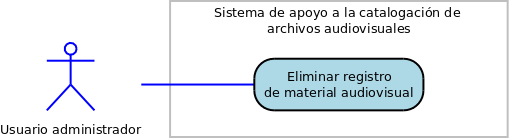
\includegraphics[width=0.8\textwidth]{CasoDeUso_Administrador_EliminarRegistro.png}
\end{figure}

% Descripción
\textbf{Descipción: } Acción que permite a un usuario borrar uno o varios archivos audiovisuales.

% Precondiciones
\textbf{Precondiciones:} Tener iniciada la sesion del usuario y haber consultado un registro audiovisual.

% Flujo Normal de Eventos (tabla)
\begin{adjustwidth}{-6em}{-6em}
	\begin{center}
		\begin{tabularx}{1.2\textwidth}{ | p{0.7cm} | X | p{0.7cm} | X | p{1.5cm} | }
			\hline
			\rowcolor{NewBlue} \multicolumn{5}{|c|}{\textbf{Flujo normal de eventos}} \\
			\hline
			\multicolumn{2}{|c|}{\textbf{Actor(es)}}	&	\multicolumn{2}{c|}{\textbf{Sistema}}	&	\textbf{Alterno} \\
			\hline
			\textbf{Paso}	&	\textbf{Acción}	&	\textbf{Paso}	&	\textbf{Acción}	&	\textbf{ID} \\
			\hline
			1 & 
			Dar clic en el botón de eliminar al consultar el archivo audiovisual.&
			2 &
			El sistema muestra un mensaje de confirmación para eliminar el archivo seleccionado&
			A1			
			\\
			\hline
			3
			&
			El usuario selecciona aceptar para borrar el archivo.
			&
			3 &
			El sistema muestra una ventana emergente diciendo que se ha eliminado el archivo audiovisual. & 
			E1 \\
			\hline
		\end{tabularx}
	\end{center}
\end{adjustwidth}

% Flujo Alterno (en caso de ser necesario)
\begin{adjustwidth}{-6em}{-6em}
	\begin{center}
		\begin{tabularx}{1.2\textwidth}{ | p{0.6cm} | X | X | }
			\hline
			\rowcolor{NewBlue} \multicolumn{3}{|c|}{\textbf{Flujo alterno de eventos}} \\
			\hline
			\textbf{ID}	&	\textbf{Descripción}	&	\textbf{Acción} \\
			\hline
			A1 &
			El usuario selecciona cancelar la eliminación del archivo audiovisual &
			El sistema cancela la eliminación y redirige a la página donde esta consultando el archivo audiovisual. \\
			\hline
		\end{tabularx}
	\end{center}
\end{adjustwidth}

% Flujo de Excepcion de Eventos (tabla)
\begin{adjustwidth}{-6em}{-6em}
	\begin{center}
		\begin{tabularx}{1.2\textwidth}{ | p{0.6cm} | X | X | }
			\hline
			\rowcolor{NewBlue} \multicolumn{3}{|c|}{\textbf{Flujo excepcional de eventos}} \\
			\hline
			\textbf{ID}	&	\textbf{Descripción}	&	\textbf{Acción} \\
			\hline
			E1 &
			No hay conexión con la base de datos. &
			El sistema devuelve un mensaje de error de conexión. \\
			\hline
		\end{tabularx}
	\end{center}
\end{adjustwidth}

% Post-condiciones
\textbf{Postcondiciones:} Se muestra en pantalla las portadas del los archivos audiovisuales sin el archivo eliminado.

% Casos de prueba para flujo normal (tabla) y su prototipo (imagen)
%\begin{figure}[H]
%	\centering
%	\includegraphics[width=0.8\textwidth]{imagen.png}
%\end{figure}

\begin{adjustwidth}{-6em}{-6em}
	\begin{center}
		\begin{tabularx}{1.2\textwidth}{ | X | X | }
			\hline
			\rowcolor{NewBlue} \multicolumn{2}{|c|}{\textbf{Casos de prueba (Flujo normal)}} \\
			\hline
			\textbf{Entradas}	&	\textbf{Resultado esperado} \\
			\hline
			Clic en el botón de eliminar. &
			El sistema muestra un mensaje de confimación para eliminar el archivo audiovisual. \\
			\hline
			Se selecciona aceptar&
			El sistema muestra un mensaje de que se ha eliminado el archivo. \\
			\hline
		\end{tabularx}
	\end{center}
\end{adjustwidth}

% Casos de prueba (Flujo alterno de eventos) [cuando es necesario]

%\begin{figure}[H]
%	\centering
%	\includegraphics[width=0.8\textwidth]{imagen.png}
%\end{figure}

\begin{adjustwidth}{-6em}{-6em}
	\begin{center}
		\begin{tabularx}{1.2\textwidth}{ | p{0.6cm} | X | X | }
			\hline
			\rowcolor{NewBlue} \multicolumn{3}{|c|}{\textbf{Caso de prueba (Flujo alterno)}} \\
			\hline
			\textbf{ID}	&	\textbf{Entrada}	&	\textbf{Resultado esperado} \\
			\hline
			A1 &
			Se selleciona la opción de cancelar. &
			El sistema cancela la eliminación redirigiendo a la página donde se esta consultando el archivo audiovisual. \\
			\hline
		\end{tabularx}
	\end{center}
\end{adjustwidth}

% Casos de prueba para excepción de eventos (tabla) y su prototipo (imagen)
%\begin{figure}[H]
%	\centering
%	\includegraphics[width=0.8\textwidth]{imagen.png}
%\end{figure}

\begin{adjustwidth}{-6em}{-6em}
	\begin{center}
		\begin{tabularx}{1.2\textwidth}{ | p{0.6cm} | X | X | }
			\hline
			\rowcolor{NewBlue} \multicolumn{3}{|c|}{\textbf{Caso de prueba (Flujo excepcional)}} \\
			\hline
			\textbf{ID}	&	\textbf{Entrada}	&	\textbf{Resultado esperado} \\
			\hline
			E1 &
			No hay conexión con la base de datos. &
			El sistema devuelve un mensaje de error de conexión. \\
			\hline
		\end{tabularx}
	\end{center}
\end{adjustwidth}

\subsubsection{Iniciar sesion como usuario del LAIS}
% Actor
\textbf{Actor:} Usuario administrador

% Imagen del diagrama específico del caso
\begin{figure}[H]
	\centering
	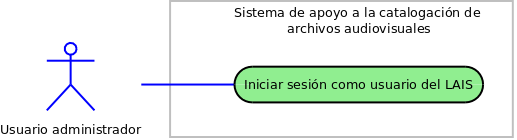
\includegraphics[width=0.8\textwidth]{CasoDeUso_Administrador_IniciarSesion.png}
\end{figure}

% Descripción
\textbf{Descipción: } Acción que permite iniciar sesión del sistema.

% Precondiciones
\textbf{Precondiciones:} Estar en cualquiera de las páginas del sistema y estar en sesión cerrada.

% Flujo Normal de Eventos (tabla)
\begin{adjustwidth}{-6em}{-6em}
	\begin{center}
		\begin{tabularx}{1.2\textwidth}{ | p{0.7cm} | X | p{0.7cm} | X | p{1.5cm} | }
			\hline
			\rowcolor{NewBlue} \multicolumn{5}{|c|}{\textbf{Flujo normal de eventos}} \\
			\hline
			\multicolumn{2}{|c|}{\textbf{Actor(es)}}	&	\multicolumn{2}{c|}{\textbf{Sistema}}	&	\textbf{Alterno} \\
			\hline
			\textbf{Paso}	&	\textbf{Acción}	&	\textbf{Paso}	&	\textbf{Acción}	&	\textbf{ID} \\
			\hline
			1 & 
			Dar clic en el botón de iniciar sesión situado en la parte superior del navegador.&
			2 &
			El sistema muestra una ventana que contiene los campos de nombre de usuario y contraseña.&\\
			\hline			
			3&
			Usuario inserta los datos correspondientes a su nombre de usuario y contraseña y da clic a iniciar sesion.&
			4&
			El sistema inicia sesión con el usuario correspondiente eliminando la ventana de iniciar sesión&
			E1,E2
			\\
			\hline
		\end{tabularx}
	\end{center}
\end{adjustwidth}

% Post-condiciones
\textbf{Postcondiciones:} El sistema cierra sesión y autoredirige al usuario a la página de inicio.

% Casos de prueba para flujo normal (tabla) y su prototipo (imagen)
%\begin{figure}[H]
%	\centering
%	\includegraphics[width=0.8\textwidth]{imagen.png}
%\end{figure}

\begin{adjustwidth}{-6em}{-6em}
	\begin{center}
		\begin{tabularx}{1.2\textwidth}{ | X | X | }
			\hline
			\rowcolor{NewBlue} \multicolumn{2}{|c|}{\textbf{Casos de prueba (Flujo normal)}} \\
			\hline
			\textbf{Entradas}	&	\textbf{Resultado esperado} \\
			\hline
			Clic en el botón de iniciar sesión. &
			El sistema muestra laa ventana de iniciar sesión. \\
			\hline
			El usuario inserta los datos correspondientes a nombre de usuario y contraseña y da clic en iniciar sesión. &
			El sistema inicia sesion con el usuario correspondiente. \\
			\hline
		\end{tabularx}
	\end{center}
\end{adjustwidth}


% Casos de prueba para excepción de eventos (tabla) y su prototipo (imagen)
%\begin{figure}[H]
%	\centering
%	\includegraphics[width=0.8\textwidth]{imagen.png}
%\end{figure}

\begin{adjustwidth}{-6em}{-6em}
	\begin{center}
		\begin{tabularx}{1.2\textwidth}{ | p{0.6cm} | X | X | }
			\hline
			\rowcolor{NewBlue} \multicolumn{3}{|c|}{\textbf{Caso de prueba (Flujo excepcional)}} \\
			\hline
			\textbf{ID}	&	\textbf{Entrada}	&	\textbf{Resultado esperado} \\
			\hline
			E1 &
			Los datos de iniciar sesión como contraseña o nombre de usuario o ambos son incorrectos. &
			El sistema devuelve un mensaje de error de los campos incorrectos. \\
			\hline
			E2 &
			No hay conexión con la base de datos. &
			El sistema devuelve un mensaje de error de conexión. \\
			\hline
		\end{tabularx}
	\end{center}
\end{adjustwidth}

\subsubsection{Cerrar sesion como usuario del LAIS}
% Actor
\textbf{Actor:} Usuario administrador

% Imagen del diagrama específico del caso
\begin{figure}[H]
	\centering
	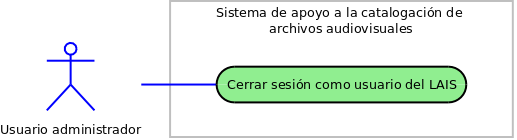
\includegraphics[width=0.8\textwidth]{CasoDeUso_Administrador_CerrarSesion.png}
\end{figure}

% Descripción
\textbf{Descipción: } Acción que permite cerrar sesión del sistema.

% Precondiciones
\textbf{Precondiciones:} Tener iniciada la sesión del usuario y estar en cualquiera de las páginas del sistema.

% Flujo Normal de Eventos (tabla)
\begin{adjustwidth}{-6em}{-6em}
	\begin{center}
		\begin{tabularx}{1.2\textwidth}{ | p{0.7cm} | X | p{0.7cm} | X | p{1.5cm} | }
			\hline
			\rowcolor{NewBlue} \multicolumn{5}{|c|}{\textbf{Flujo normal de eventos}} \\
			\hline
			\multicolumn{2}{|c|}{\textbf{Actor(es)}}	&	\multicolumn{2}{c|}{\textbf{Sistema}}	&	\textbf{Alterno} \\
			\hline
			\textbf{Paso}	&	\textbf{Acción}	&	\textbf{Paso}	&	\textbf{Acción}	&	\textbf{ID} \\
			\hline
			1 & 
			Dar clic en el botón de cerrar sesión situado en la parte superior del navegador.&
			2 &
			El sistema cierra sesión redirigiendo a la página de inicio.&			
			\\
			\hline
		\end{tabularx}
	\end{center}
\end{adjustwidth}

% Post-condiciones
\textbf{Postcondiciones:} El sistema cierra sesión y autoredirige al usuario a la página de inicio.

% Casos de prueba para flujo normal (tabla) y su prototipo (imagen)
%\begin{figure}[H]
%	\centering
%	\includegraphics[width=0.8\textwidth]{imagen.png}
%\end{figure}

\begin{adjustwidth}{-6em}{-6em}
	\begin{center}
		\begin{tabularx}{1.2\textwidth}{ | X | X | }
			\hline
			\rowcolor{NewBlue} \multicolumn{2}{|c|}{\textbf{Casos de prueba (Flujo normal)}} \\
			\hline
			\textbf{Entradas}	&	\textbf{Resultado esperado} \\
			\hline
			Clic en el botón de cerrar sesión. &
			El sistema cierra sesión. \\
			\hline
		\end{tabularx}
	\end{center}
\end{adjustwidth}

% Casos de prueba (Flujo alterno de eventos) [cuando es necesario]

%\begin{figure}[H]
%	\centering
%	\includegraphics[width=0.8\textwidth]{imagen.png}
%\end{figure}

\begin{adjustwidth}{-6em}{-6em}
	\begin{center}
		\begin{tabularx}{1.2\textwidth}{ | p{0.6cm} | X | X | }
			\hline
			\rowcolor{NewBlue} \multicolumn{3}{|c|}{\textbf{Caso de prueba (Flujo alterno)}} \\
			\hline
			\textbf{ID}	&	\textbf{Entrada}	&	\textbf{Resultado esperado} \\
			\hline
			A1 &
			Se selleciona la opción de cancelar. &
			El sistema cancela la eliminación redirigiendo a la página donde se esta consultando el archivo audiovisual. \\
			\hline
		\end{tabularx}
	\end{center}
\end{adjustwidth}

% Casos de prueba para excepción de eventos (tabla) y su prototipo (imagen)
%\begin{figure}[H]
%	\centering
%	\includegraphics[width=0.8\textwidth]{imagen.png}
%\end{figure}

\begin{adjustwidth}{-6em}{-6em}
	\begin{center}
		\begin{tabularx}{1.2\textwidth}{ | p{0.6cm} | X | X | }
			\hline
			\rowcolor{NewBlue} \multicolumn{3}{|c|}{\textbf{Caso de prueba (Flujo excepcional)}} \\
			\hline
			\textbf{ID}	&	\textbf{Entrada}	&	\textbf{Resultado esperado} \\
			\hline
			E1 &
			No hay conexión con la base de datos. &
			El sistema devuelve un mensaje de error de conexión. \\
			\hline
		\end{tabularx}
	\end{center}
\end{adjustwidth}

\subsubsection{Agregar usuario al sistema}
% Actor
\textbf{Actor:} Usuario administrador

% Imagen del diagrama específico del caso
\begin{figure}[H]
	\centering
	\includegraphics[width=0.8\textwidth]{CasoDeUso_Administrador_AdministracionDeUsuarios.png}
\end{figure}

% Descripción
\textbf{Descipción: } Acción que permite a un administrador registrar a otro usuario. El tipo de usuario que se agrega comúnmente es un usuario con permisos para agregar u otro administrador.

% Precondiciones
\textbf{Precondiciones:} Ser un usuario con permisos de administrador y tener iniciada la sesión.

% Flujo Normal de Eventos (tabla)
\begin{adjustwidth}{-6em}{-6em}
	\begin{center}
		\begin{tabularx}{1.2\textwidth}{ | p{0.7cm} | X | p{0.7cm} | X | p{1.5cm} | }
			\hline
			\rowcolor{NewBlue} \multicolumn{5}{|c|}{\textbf{Flujo normal de eventos}} \\
			\hline
			\multicolumn{2}{|c|}{\textbf{Actor(es)}}	&	\multicolumn{2}{c|}{\textbf{Sistema}}	&	\textbf{Alterno} \\
			\hline
			\textbf{Paso}	&	\textbf{Acción}	&	\textbf{Paso}	&	\textbf{Acción}	&	\textbf{ID} \\
			\hline
			1 & 
			El usuario da clic sobre su nombre de usuario en la barra superior de la página.&
			2 &
			El sistema despliega un pequeño recuadro donde se muestra la opción ``Administración''. &
			
			\\
			\hline
			3 & 
			El usuario da clic en la opción ``Administración''.&
			4 &
			El sistema envia a la página de Administración de usuarios donde se muestra un breve formulario junto con la lista de los usuarios registrados.&
			E1
			\\
			\hline
			5 & 
			El usuario llenará los campos del formulario con la información solicitada y da clic en el botón \textit{Enviar}.&
			6 &
			El sistema envia los datos a la base de datos y muestra un mensaje de éxito. Se recarga la página para enlistar al nuevo usuario registrado.&
			E1,E2
			\\
			\hline
		\end{tabularx}
	\end{center}
\end{adjustwidth}

% Flujo de Excepcion de Eventos (tabla)
\begin{adjustwidth}{-6em}{-6em}
	\begin{center}
		\begin{tabularx}{1.2\textwidth}{ | p{0.6cm} | X | X | }
			\hline
			\rowcolor{NewBlue} \multicolumn{3}{|c|}{\textbf{Flujo excepcional de eventos}} \\
			\hline
			\textbf{ID}	&	\textbf{Descripción}	&	\textbf{Acción} \\
			\hline
			E1 &
			No hay conexión con la base de datos. &
			El sistema devuelve un mensaje de error de conexión. \\
			\hline
			E2 &
			Los campos del usuario no estan llenados correctamente. &
			El sistema muestra un mensaje error por cada campo incorrecto y desactiva el botón de agregar. \\
			\hline
		\end{tabularx}
	\end{center}
\end{adjustwidth}

% Post-condiciones
\textbf{Postcondiciones:} Se registra el nuevo usuario con los permisos establecidos y está listo para iniciar sesión.

% Casos de prueba para flujo normal (tabla) y su prototipo (imagen)
%\begin{figure}[H]
%	\centering
%	\includegraphics[width=0.8\textwidth]{imagen.png}
%\end{figure}

\begin{adjustwidth}{-6em}{-6em}
	\begin{center}
		\begin{tabularx}{1.2\textwidth}{ | X | X | }
			\hline
			\rowcolor{NewBlue} \multicolumn{2}{|c|}{\textbf{Casos de prueba (Flujo normal)}} \\
			\hline
			\textbf{Entradas}	&	\textbf{Resultado esperado} \\
			\hline
			Seleccionar el nombre de usuario en la barra superior de la página.&
			El sistema despliega un pequeño recuadro donde se muestra la opción ``Administración''.\\
			\hline
			El usuario da clic en la opción ``Administración''.&
			El sistema muestra el formulario con sus respectivos campos a llenar para registrar nuevo usuario. \\
			\hline
			El usuario inserta la información en los campos necesarios y da clic en el botón \textit{Enviar}.&
			El sistema manda un mensaje de que se ha agregado con exíto un nuevo usuario.\\
			\hline
		\end{tabularx}
	\end{center}
\end{adjustwidth}

% Casos de prueba para excepción de eventos (tabla) y su prototipo (imagen)
%\begin{figure}[H]
%	\centering
%	\includegraphics[width=0.8\textwidth]{imagen.png}
%\end{figure}

\begin{adjustwidth}{-6em}{-6em}
	\begin{center}
		\begin{tabularx}{1.2\textwidth}{ | p{0.6cm} | X | X | }
			\hline
			\rowcolor{NewBlue} \multicolumn{3}{|c|}{\textbf{Caso de prueba (Flujo excepcional)}} \\
			\hline
			\textbf{ID}	&	\textbf{Entrada}	&	\textbf{Resultado esperado} \\
			\hline
			E1 &
			No hay conexión con la base de datos. &
			El sistema devuelve un mensaje de error de conexión. \\
			\hline
			E2 &
			Los datos insertados en los campos del formulario no son correctos. &
			El sistema muestra un mensaje de error por cada campo incorrecto y desactiva el botón \textit{Enviar}. \\
			\hline
		\end{tabularx}
	\end{center}
\end{adjustwidth}

\subsubsection{Editar usuario del sistema}
% Actor
\textbf{Actor:} Usuario administrador

% Imagen del diagrama específico del caso
\begin{figure}[H]
	\centering
	\includegraphics[width=0.8\textwidth]{CasoDeUso_Administrador_AdministracionDeUsuarios.png}
\end{figure}

% Descripción
\textbf{Descipción: } Acción que permite a un administrador editar la información (nombre y contraseña) o permisos de un usuario registrado (incluyendo al mismo usuario).

% Precondiciones
\textbf{Precondiciones:} Ser un usuario con permisos de administrador y tener iniciada la sesión.

% Flujo Normal de Eventos (tabla)
\begin{adjustwidth}{-6em}{-6em}
	\begin{center}
		\begin{tabularx}{1.2\textwidth}{ | p{0.7cm} | X | p{0.7cm} | X | p{1.5cm} | }
			\hline
			\rowcolor{NewBlue} \multicolumn{5}{|c|}{\textbf{Flujo normal de eventos}} \\
			\hline
			\multicolumn{2}{|c|}{\textbf{Actor(es)}}	&	\multicolumn{2}{c|}{\textbf{Sistema}}	&	\textbf{Alterno} \\
			\hline
			\textbf{Paso}	&	\textbf{Acción}	&	\textbf{Paso}	&	\textbf{Acción}	&	\textbf{ID} \\
			\hline
			1 & 
			El usuario da clic sobre su nombre de usuario en la barra superior de la página.&
			2 &
			El sistema despliega un pequeño recuadro donde se muestra la opción ``Administración''. &
			
			\\
			\hline
			3 & 
			El usuario da clic en la opción ``Administración''.&
			4 &
			El sistema envia a la página de Administración de usuarios donde se muestra un breve formulario junto con la lista de los usuarios registrados (del lado derecho de cada usuario incluye un botón de edición).&
			E1
			\\
			\hline
			5 & 
			El usuario identifica al usuario en la lista y da clic en el botón \textit{Editar}&
			6 &
			El sistema pide la información a la base de datos y agrega dicha información en el formulario de la parte superior.&
			E1
			\\
			\hline
			7 & 
			El usuario modificará los campos del formulario con la información necesaria y da clic en el botón \textit{Actualizar}.&
			8 &
			El sistema envia los datos a la base de datos y muestra un mensaje de éxito. Se recarga la página para enlistar al usuario con la nueva información.&
			E1,E2
			\\
			\hline
		\end{tabularx}
	\end{center}
\end{adjustwidth}

% Flujo de Excepcion de Eventos (tabla)
\begin{adjustwidth}{-6em}{-6em}
	\begin{center}
		\begin{tabularx}{1.2\textwidth}{ | p{0.6cm} | X | X | }
			\hline
			\rowcolor{NewBlue} \multicolumn{3}{|c|}{\textbf{Flujo excepcional de eventos}} \\
			\hline
			\textbf{ID}	&	\textbf{Descripción}	&	\textbf{Acción} \\
			\hline
			E1 &
			No hay conexión con la base de datos. &
			El sistema devuelve un mensaje de error de conexión. \\
			\hline
			E2 &
			Los campos del usuario no estan llenados correctamente. &
			El sistema muestra un mensaje error por cada campo incorrecto y desactiva el botón de agregar. \\
			\hline
		\end{tabularx}
	\end{center}
\end{adjustwidth}

% Post-condiciones
\textbf{Postcondiciones:} Se reflejan inmediatamente los cambios del usuario: cambiar nombre de usuario, contraseña o tipo de privilegios.

% Casos de prueba para flujo normal (tabla) y su prototipo (imagen)
%\begin{figure}[H]
%	\centering
%	\includegraphics[width=0.8\textwidth]{imagen.png}
%\end{figure}

\begin{adjustwidth}{-6em}{-6em}
	\begin{center}
		\begin{tabularx}{1.2\textwidth}{ | X | X | }
			\hline
			\rowcolor{NewBlue} \multicolumn{2}{|c|}{\textbf{Casos de prueba (Flujo normal)}} \\
			\hline
			\textbf{Entradas}	&	\textbf{Resultado esperado} \\
			\hline
			Seleccionar el nombre de usuario en la barra superior de la página.&
			El sistema despliega un pequeño recuadro donde se muestra la opción ``Administración''.\\
			\hline
			El usuario da clic en la opción ``Administración''.&
			El sistema muestra en la parte inferior una lista con los usuarios del sistema, incluyendo un botón de edición al lado derecho de cada usuario. \\
			\hline
			El usuario identifica al usuario en la lista y da clic en el botón \textit{Editar}&
			El sistema agrega la información actual del usuario en el formulario en la parte superior de la página. \\
			\hline
			El usuario modifica la información en los campos necesarios y da clic en el botón \textit{Actualizar}.&
			El sistema manda un mensaje de que se ha modificado con éxito al usuario.\\
			\hline
		\end{tabularx}
	\end{center}
\end{adjustwidth}

			
% Casos de prueba para excepción de eventos (tabla) y su prototipo (imagen)
%\begin{figure}[H]
%	\centering
%	\includegraphics[width=0.8\textwidth]{imagen.png}
%\end{figure}

\begin{adjustwidth}{-6em}{-6em}
	\begin{center}
		\begin{tabularx}{1.2\textwidth}{ | p{0.6cm} | X | X | }
			\hline
			\rowcolor{NewBlue} \multicolumn{3}{|c|}{\textbf{Caso de prueba (Flujo excepcional)}} \\
			\hline
			\textbf{ID}	&	\textbf{Entrada}	&	\textbf{Resultado esperado} \\
			\hline
			E1 &
			No hay conexión con la base de datos. &
			El sistema devuelve un mensaje de error de conexión. \\
			\hline
			E2 &
			Los datos insertados en los campos del formulario no son correctos. &
			El sistema muestra un mensaje de error por cada campo incorrecto y desactiva el botón \textit{Actualizar}. \\
			\hline
		\end{tabularx}
	\end{center}
\end{adjustwidth}


\subsubsection{Eliminar usuario del sistema}
% Actor
\textbf{Actor:} Usuario administrador

% Imagen del diagrama específico del caso
\begin{figure}[H]
	\centering
	\includegraphics[width=0.8\textwidth]{CasoDeUso_Administrador_AdministracionDeUsuarios.png}
\end{figure}

% Descripción
\textbf{Descipción: } Acción que permite a un administrador eliminar a un usuario registrado en el sistema.

% Precondiciones
\textbf{Precondiciones:} Ser un usuario con permisos de administrador y tener iniciada la sesión.

% Flujo Normal de Eventos (tabla)
\begin{adjustwidth}{-6em}{-6em}
	\begin{center}
		\begin{tabularx}{1.2\textwidth}{ | p{0.7cm} | X | p{0.7cm} | X | p{1.5cm} | }
			\hline
			\rowcolor{NewBlue} \multicolumn{5}{|c|}{\textbf{Flujo normal de eventos}} \\
			\hline
			\multicolumn{2}{|c|}{\textbf{Actor(es)}}	&	\multicolumn{2}{c|}{\textbf{Sistema}}	&	\textbf{Alterno} \\
			\hline
			\textbf{Paso}	&	\textbf{Acción}	&	\textbf{Paso}	&	\textbf{Acción}	&	\textbf{ID} \\
			\hline
			1 & 
			El usuario da clic sobre su nombre de usuario en la barra superior de la página.&
			2 &
			El sistema despliega un pequeño recuadro donde se muestra la opción ``Administración''. &
			
			\\
			\hline
			3 & 
			El usuario da clic en la opción ``Administración''.&
			4 &
			El sistema envia a la página de Administración de usuarios donde se muestra un breve formulario junto con la lista de los usuarios registrados (del lado derecho de cada usuario incluye un botón de borrar).&
			E1
			\\
			\hline
			5 & 
			El usuario identifica al usuario en la lista y da clic en el botón \textit{Borrar}&
			6 &
			El sistema muestra un mensaje de confirmación para eliminar al usuario seleccionado.&
			A1
			\\
			7 &
			El usuario selecciona aceptar para borrar al usuario del sistema. &
			8 &
			El sistema muestra un mensaje de éxito. Se recarga la página para mostrar que el usuario ya no aparece entre los usuarios registrados.& 
			E1 \\
			\hline
		\end{tabularx}
	\end{center}
\end{adjustwidth}

% Flujo Alterno (en caso de ser necesario)
\begin{adjustwidth}{-6em}{-6em}
	\begin{center}
		\begin{tabularx}{1.2\textwidth}{ | p{0.6cm} | X | X | }
			\hline
			\rowcolor{NewBlue} \multicolumn{3}{|c|}{\textbf{Flujo alterno de eventos}} \\
			\hline
			\textbf{ID}	&	\textbf{Descripción}	&	\textbf{Acción} \\
			\hline
			A1 &
			El usuario selecciona cancelar la eliminación del usuario &
			El sistema cancela la eliminación. \\
			\hline
		\end{tabularx}
	\end{center}
\end{adjustwidth}

% Flujo de Excepcion de Eventos (tabla)
\begin{adjustwidth}{-6em}{-6em}
	\begin{center}
		\begin{tabularx}{1.2\textwidth}{ | p{0.6cm} | X | X | }
			\hline
			\rowcolor{NewBlue} \multicolumn{3}{|c|}{\textbf{Flujo excepcional de eventos}} \\
			\hline
			\textbf{ID}	&	\textbf{Descripción}	&	\textbf{Acción} \\
			\hline
			E1 &
			No hay conexión con la base de datos. &
			El sistema devuelve un mensaje de error de conexión. \\
			\hline
			E2 &
			Los campos del usuario no estan llenados correctamente. &
			El sistema muestra un mensaje error por cada campo incorrecto y desactiva el botón de agregar. \\
			\hline
		\end{tabularx}
	\end{center}
\end{adjustwidth}

% Post-condiciones
\textbf{Postcondiciones:} El usuario eliminado ya no tiene permitido el acceder al sistema ni será mostrado en la lista de usuarios registrados.

% Casos de prueba para flujo normal (tabla) y su prototipo (imagen)
%\begin{figure}[H]
%	\centering
%	\includegraphics[width=0.8\textwidth]{imagen.png}
%\end{figure}

\begin{adjustwidth}{-6em}{-6em}
	\begin{center}
		\begin{tabularx}{1.2\textwidth}{ | X | X | }
			\hline
			\rowcolor{NewBlue} \multicolumn{2}{|c|}{\textbf{Casos de prueba (Flujo normal)}} \\
			\hline
			\textbf{Entradas}	&	\textbf{Resultado esperado} \\
			\hline
			Seleccionar el nombre de usuario en la barra superior de la página.&
			El sistema despliega un pequeño recuadro donde se muestra la opción ``Administración''.\\
			\hline
			El usuario da clic en la opción ``Administración''.&
			El sistema muestra en la parte inferior una lista con los usuarios del sistema, incluyendo un botón de borrado al lado derecho de cada usuario. \\
			\hline
			El usuario identifica al usuario en la lista y da clic en el botón \textit{Borrar}&
			El sistema muestra un mensaje de confirmación para eliminar al usuario seleccionado.\\
			\hline
			Se confirma la eliminación del usuario.&
			El sistema manda un mensaje de que se ha elminado con éxito al usuario.\\
			\hline
		\end{tabularx}
	\end{center}
\end{adjustwidth}

% Casos de prueba (Flujo alterno de eventos) [cuando es necesario]

%\begin{figure}[H]
%	\centering
%	\includegraphics[width=0.8\textwidth]{imagen.png}
%\end{figure}

\begin{adjustwidth}{-6em}{-6em}
	\begin{center}
		\begin{tabularx}{1.2\textwidth}{ | p{0.6cm} | X | X | }
			\hline
			\rowcolor{NewBlue} \multicolumn{3}{|c|}{\textbf{Caso de prueba (Flujo alterno)}} \\
			\hline
			\textbf{ID}	&	\textbf{Entrada}	&	\textbf{Resultado esperado} \\
			\hline
			A1 &
			Se selleciona la opción de cancelar. &
			El sistema cancela la eliminación y se muestra nuevamente la página de administración de usuarios. \\
			\hline
		\end{tabularx}
	\end{center}
\end{adjustwidth}
			
% Casos de prueba para excepción de eventos (tabla) y su prototipo (imagen)
%\begin{figure}[H]
%	\centering
%	\includegraphics[width=0.8\textwidth]{imagen.png}
%\end{figure}

\begin{adjustwidth}{-6em}{-6em}
	\begin{center}
		\begin{tabularx}{1.2\textwidth}{ | p{0.6cm} | X | X | }
			\hline
			\rowcolor{NewBlue} \multicolumn{3}{|c|}{\textbf{Caso de prueba (Flujo excepcional)}} \\
			\hline
			\textbf{ID}	&	\textbf{Entrada}	&	\textbf{Resultado esperado} \\
			\hline
			E1 &
			No hay conexión con la base de datos. &
			El sistema devuelve un mensaje de error de conexión. \\
			\hline
			E2 &
			Los datos insertados en los campos del formulario no son correctos. &
			El sistema muestra un mensaje de error por cada campo incorrecto y desactiva el botón \textit{Actualizar}. \\
			\hline
		\end{tabularx}
	\end{center}
\end{adjustwidth}

\end{document}